\documentclass[aspectratio=169]{ctexbeamer}
\usepackage[bluetheme]{ustcbeamer}
\usepackage{blocktheme}
\input{ustctheme.tex}
% \setCJKmainfont{SimSun}[BoldFont=SimHei, ItalicFont=KaiTi]
\title[AI图像识别技术及其应用]{AI图像识别技术及其应用}
\author[苏家望, 李越衡, 崔俊熙]{报告人: 苏家望, 李越衡, 崔俊熙}
\institute[USTC]{中国科学技术大学, 少年班学院}
\date{\today}
\begin{document}
\maketitleframe

\begin{frame}
	\frametitle{大纲}
	\tableofcontents[hideallsubsections]
\end{frame}

\AtBeginSection[]{
	\setbeamertemplate{footline}[footlineoff]
	\begin{frame}
		\frametitle{大纲}
		\tableofcontents[currentsection, subsectionstyle=show/show/hide]
	\end{frame}
	\setbeamertemplate{footline}[footlineon]
}

\AtBeginSubsection[]{
	\setbeamertemplate{footline}[footlineoff]
	\begin{frame}
		\frametitle{大纲}
		\tableofcontents[currentsection, subsectionstyle=show/shaded/hide]
	\end{frame}
	\setbeamertemplate{footline}[footlineon]
}

\section[技术概述]{AI图像识别的技术概述}

% \begin{frame}
%     \frametitle{技术定义}
%     \begin{block}{核心原理}
%         AI图像识别的目标是让计算机``看懂图片''.
%         通过学习大量图像数据, 计算机可以逐渐学会识别物体, 例如区分猫和狗, 识别道路标志或判断图片中的人物.

%         例如Google的\textbf{Google Photos}可以自动识别照片中的人物和地点, 并进行智能分类.
%     \end{block}
%     \begin{block}{性能指标}
%         评价图像识别系统时, 通常关注识别的准确率和处理速度.

%         例如手机中的人脸解锁系统通常需要在不到一秒的时间内完成识别, 同时保持较高的准确率.
%     \end{block}
%     \begin{block}{与传统方法区别}
%         传统图像处理依赖人工设计规则, 例如手动寻找图像中的边缘或颜色.

%         而AI方法可以通过学习大量数据自动总结规律, 因此在复杂场景中往往表现更好, 例如自动驾驶中的道路识别.
%         \end{block}
% \end{frame}

\begin{frame}
	\frametitle{发展起源}

	\begin{columns}[t]
		\begin{column}{0.3\linewidth}
			\begin{block}{早期探索}
				20世纪中期, 科学家提出了最早的神经网络模型, 希望让计算机能够识别简单图形, 例如直线或几何形状.
				\begin{figure}
					\centering
					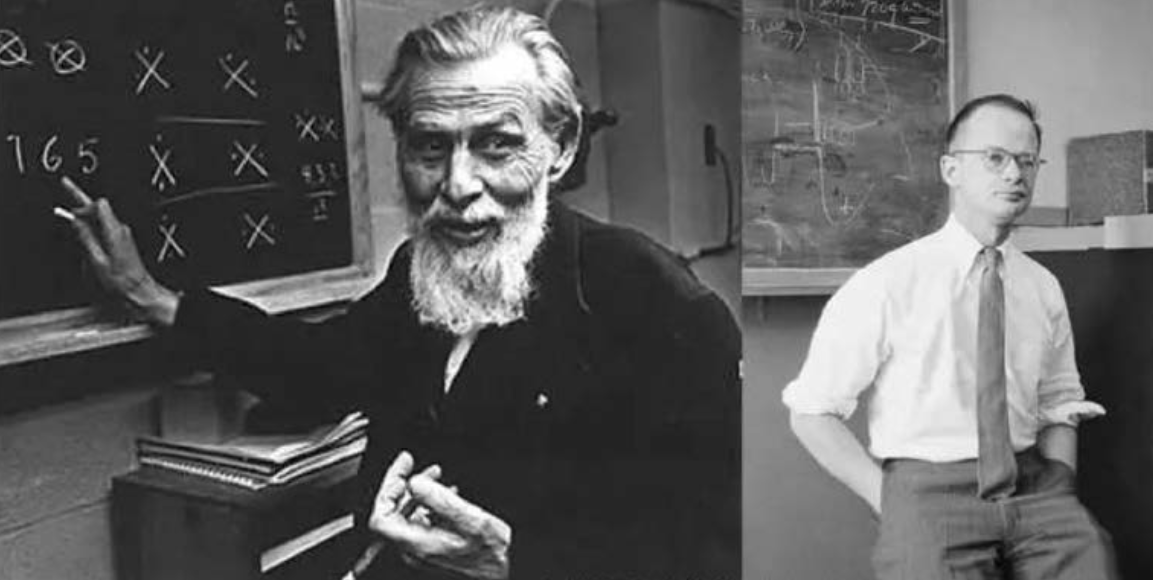
\includegraphics[width=0.8\linewidth]{figures/fig1.png}
				\end{figure}
			\end{block}
		\end{column}
		\begin{column}{0.3\linewidth}
			\begin{block}{算法发展}
				20世纪末, 研究人员开始利用神经网络识别手写数字. 例如美国AT\&T实验室的研究团队开发的系统, 可以识别银行支票上的数字.
				\begin{figure}
					\centering
					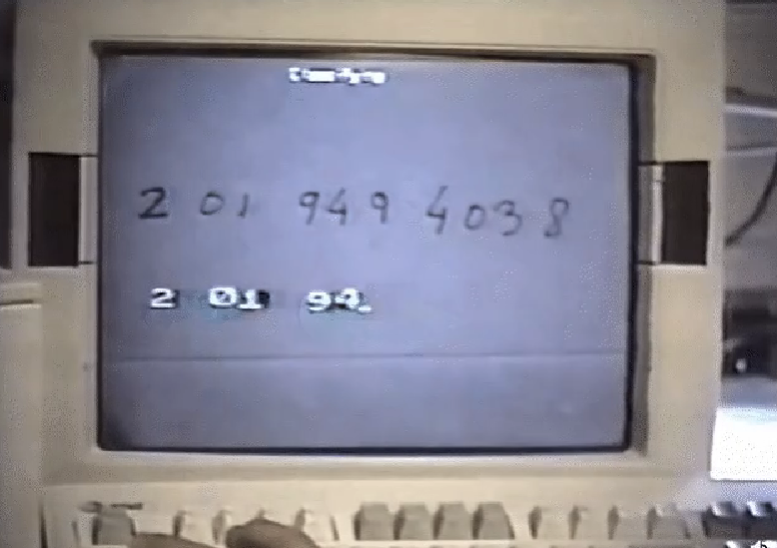
\includegraphics[width=0.8\linewidth]{figures/fig2.png}
				\end{figure}
			\end{block}
		\end{column}
		\begin{column}{0.3\linewidth}
			\begin{block}{深度学习时代}
				Geoffrey Hinton 和 John Hopfield 共同获得 2024 年诺贝尔物理学奖以表彰他们利用人工神经网络进行机器学习的基础发现和发明.
				\begin{figure}
					\centering
					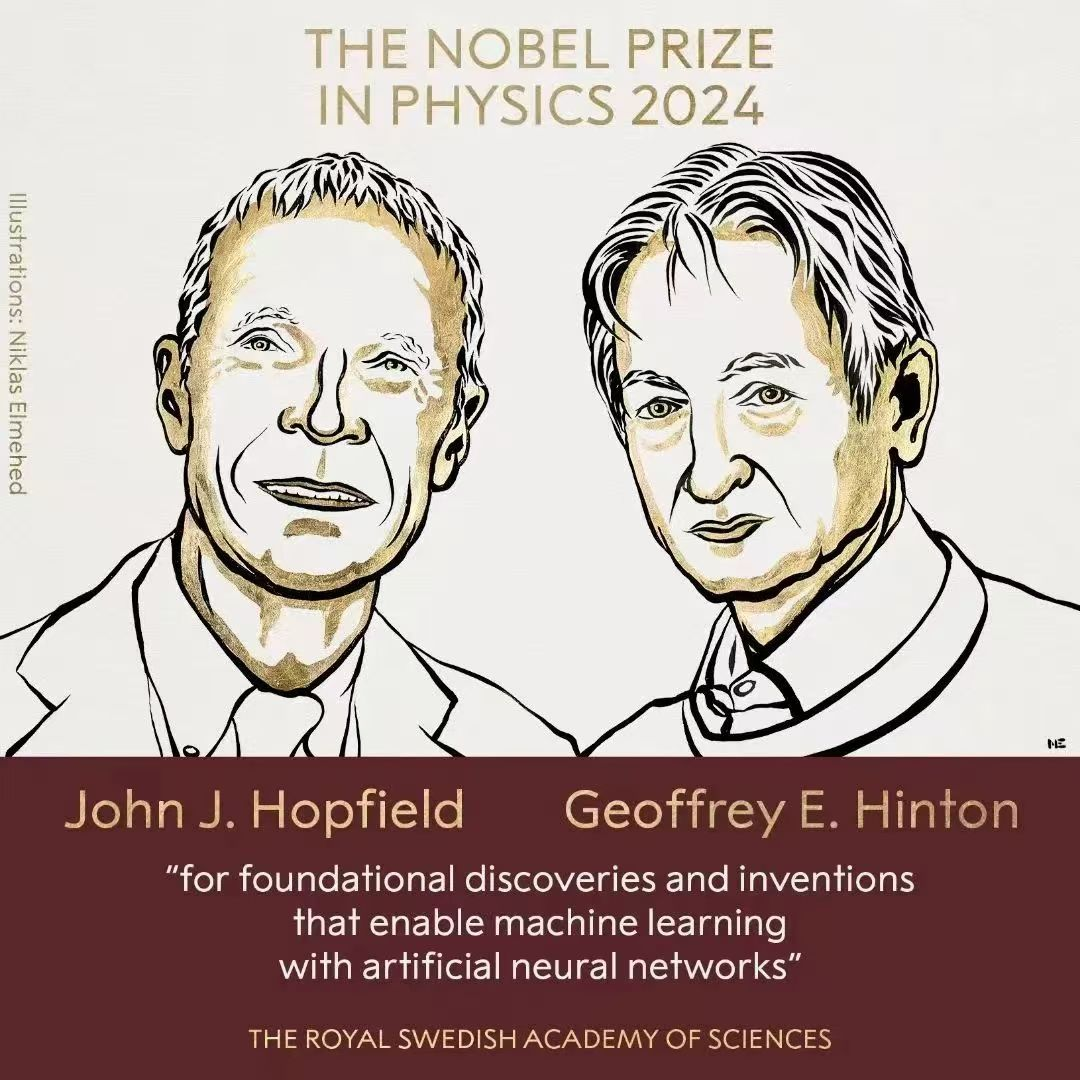
\includegraphics[width=0.7\linewidth]{figures/fig3.jpg}
				\end{figure}
			\end{block}
		\end{column}
	\end{columns}
\end{frame}

\section[技术原理]{AI图像识别的技术原理}

\begin{frame}
	\frametitle{数据采集与预处理}
	\begin{columns}[t]
		\begin{column}{0.3\linewidth}
			\begin{block}{图像数据采集}
				首先需要收集大量图片, 例如街道场景, 动物照片或医疗影像.

				例如自动驾驶公司会收集大量道路图像, 用来训练汽车识别车道线, 行人和交通标志.
			\end{block}
		\end{column}
		\begin{column}{0.3\linewidth}
			\begin{block}{图像预处理}
				在训练之前, 通常需要对图片进行简单处理, 例如去除噪声, 统一尺寸或调整亮度, 使数据更加清晰和一致.
			\end{block}
		\end{column}
		\begin{column}{0.3\linewidth}
			\begin{block}{数据增强}
				通过旋转, 裁剪或改变亮度等方式生成新的训练样本.

				例如一张道路图片可以旋转或翻转生成多个样本, 从而让模型学到更多不同情况.
			\end{block}
		\end{column}
	\end{columns}
\end{frame}

\begin{frame}
	\frametitle{层级特征学习}
	\begin{columns}[t]
		\begin{column}{0.3\linewidth}
			\begin{block}{浅层特征}
				网络浅层检测基础视觉元素, 如边缘, 角点和颜色块.

				这些低级特征与具体任务无关, 在不同数据集中具有通用性.
			\end{block}
		\end{column}
		\begin{column}{0.3\linewidth}
			\begin{block}{中层特征}
				将浅层边缘组合为纹理, 局部形状和图案.

				例如检测车轮的圆形轮廓, 眼睛的椭圆形等更复杂的结构.
			\end{block}
		\end{column}
		\begin{column}{0.3\linewidth}
			\begin{block}{高层语义特征}
				网络最深层的神经元对应高级语义概念, 如人脸, 车辆, 文字等.

				层数越深, 特征越抽象, 与具体分类目标的关联越强.
			\end{block}
		\end{column}
	\end{columns}
\end{frame}

\begin{frame}
	\frametitle{前向传播与反向传播}
	\begin{columns}[t]
		\begin{column}{0.3\linewidth}
			\begin{block}{前向传播}
				输入图像经过多层卷积, 池化等操作, 逐层提取特征, 最终由全连接层输出分类结果.

				每一层通过非线性激活函数引入表达能力.
			\end{block}
		\end{column}
		\begin{column}{0.3\linewidth}
			\begin{block}{损失函数}
				将网络输出的预测值与真实标签进行比较, 计算损失.

				交叉熵损失常用于分类任务: 预测越准确, 损失值越小.
			\end{block}
		\end{column}
		\begin{column}{0.3\linewidth}
			\begin{block}{反向传播与梯度下降}
				通过链式法则从输出层逐层向前计算每个参数的梯度.

				利用梯度下降更新权重: $w \leftarrow w - \eta \cdot \nabla L$, 使损失逐步降低.
			\end{block}
		\end{column}
	\end{columns}
\end{frame}

\begin{frame}
	\frametitle{主流网络架构}
	\begin{columns}[t]
		\begin{column}{0.3\linewidth}
			\begin{block}{卷积神经网络 (CNN)}
				通过卷积核在图像上滑动提取局部特征, 参数共享大幅减少参数量.

				LeNet手写数字识别, AlexNet在ImageNet竞赛中取得突破.
			\end{block}
		\end{column}
		\begin{column}{0.3\linewidth}
			\begin{block}{残差网络 (ResNet)}
				引入跳跃连接 (skip connection) , 使梯度可以直接流向浅层.

				解决了深层网络的退化问题, 使百层以上的网络训练成为可能.
			\end{block}
		\end{column}
		\begin{column}{0.3\linewidth}
			\begin{block}{Vision Transformer (ViT)}
				将图像分割为固定大小的块, 转化为序列输入Transformer.

				在ImageNet上超越同规模CNN, 推动了计算机视觉领域的范式转变.
			\end{block}
		\end{column}
	\end{columns}
\end{frame}

\section[发展现状]{AI图像识别的发展现状}

\begin{frame}
	\frametitle{市场规模与增长}
	\begin{columns}[t]
		\begin{column}{0.55\linewidth}
			\begin{center}
				\begin{tikzpicture}[scale=0.65]
					% 坐标轴
					\draw[->, thick] (0,0) -- (11,0) node[above] {\tiny 年份};
					\draw[->, thick] (0,0) -- (0,6.5) node[right] {\tiny 亿美元};
					% x轴刻度
					\foreach \x/\year in {0/2015,1/2017,2/2019,3/2021,5/2025,6/2027,7/2029,8/2031}
					\draw (\x*1.2,0) node[below] {\tiny \year};
					% y轴刻度
					\foreach \y/\val in {0/0,1/100,2/200,3/300,4/400,5/500,6/600}
					\draw (0,\y) node[left] {\tiny \val};
					% 网格线
					\foreach \y in {1,..., 6}
					\draw[gray!20] (0,\y) -- (9.6,\y);
					% 数据点: 2015~2030 (亿美元) 
					\draw[themecolor, line width=1.8pt]
					(0*1.2,0.45) -- % 2015: 45
					(0.5*1.2,0.58) -- % 2016: 58
					(1*1.2,0.75) -- % 2017: 75
					(1.5*1.2,0.95) -- % 2018: 95
					(2*1.2,1.20) -- % 2019: 120
					(2.5*1.2,1.15) -- % 2020: 115
					(3*1.2,1.40) -- % 2021: 140
					(3.5*1.2,1.70) -- % 2022: 170
					(4*1.2,2.00) -- % 2023: 200
					(4.5*1.2,2.30) -- % 2024: 230
					(5*1.2,2.65) -- % 2025: 265
					(5.5*1.2,3.05) -- % 2026: 305
					(6*1.2,3.50) -- % 2027: 350
					(6.5*1.2,4.03) -- % 2028: 403
					(7*1.2,4.63) -- % 2029: 463
					(7.5*1.2,5.32); % 2030: 532
					% 描点
					\foreach \x/\y in {0/0.45,0.5/0.58,1/0.75,1.5/0.95,2/1.20,2.5/1.15,3/1.40,3.5/1.70,4/2.00,4.5/2.30,5/2.65,5.5/3.05,6/3.50,6.5/4.03,7/4.63,7.5/5.32}
					\filldraw[themecolor] (\x*1.2,\y) circle (2.5pt);
					% 数据标注
					\draw[dashed, themecolor!50] (4*1.2,2.00) -- (4*1.2,0) node[below] {\tiny \textbf{2023}};
					\draw[dashed, themecolor!50] (7.5*1.2,5.32) -- (7.5*1.2,-0.5) node[below] {\tiny \textbf{2030}};
					\node[above] at (4*1.2,2.00) {\tiny \textbf{200亿}};
					\node[above] at (7.5*1.2,5.32) {\tiny \textbf{500亿}};
					% 图例
					\draw[themecolor, line width=1.8pt] (1,6.2) -- (2,6.2);
					\node[right] at (2,6.2) {\tiny 全球计算机视觉市场规模};
				\end{tikzpicture}
			\end{center}
		\end{column}
		\begin{column}{0.4\linewidth}
			\begin{block}{全球市场}
				全球计算机视觉市场规模在2023年已超过\textbf{200亿美元}, 预计2030年将突破\textbf{500亿美元}, 年复合增长率超过15\%.
			\end{block}
			\begin{block}{主要驱动力}
				算力成本下降与数据规模爆发推动AI图像识别在各行各业加速落地, 广泛应用于自动驾驶, 医疗影像和人脸识别等领域.
			\end{block}
		\end{column}
	\end{columns}
\end{frame}

\begin{frame}
	\frametitle{医疗影像诊断}
	\begin{columns}
		\begin{column}{0.5\linewidth}
			\begin{figure}
				\centering
				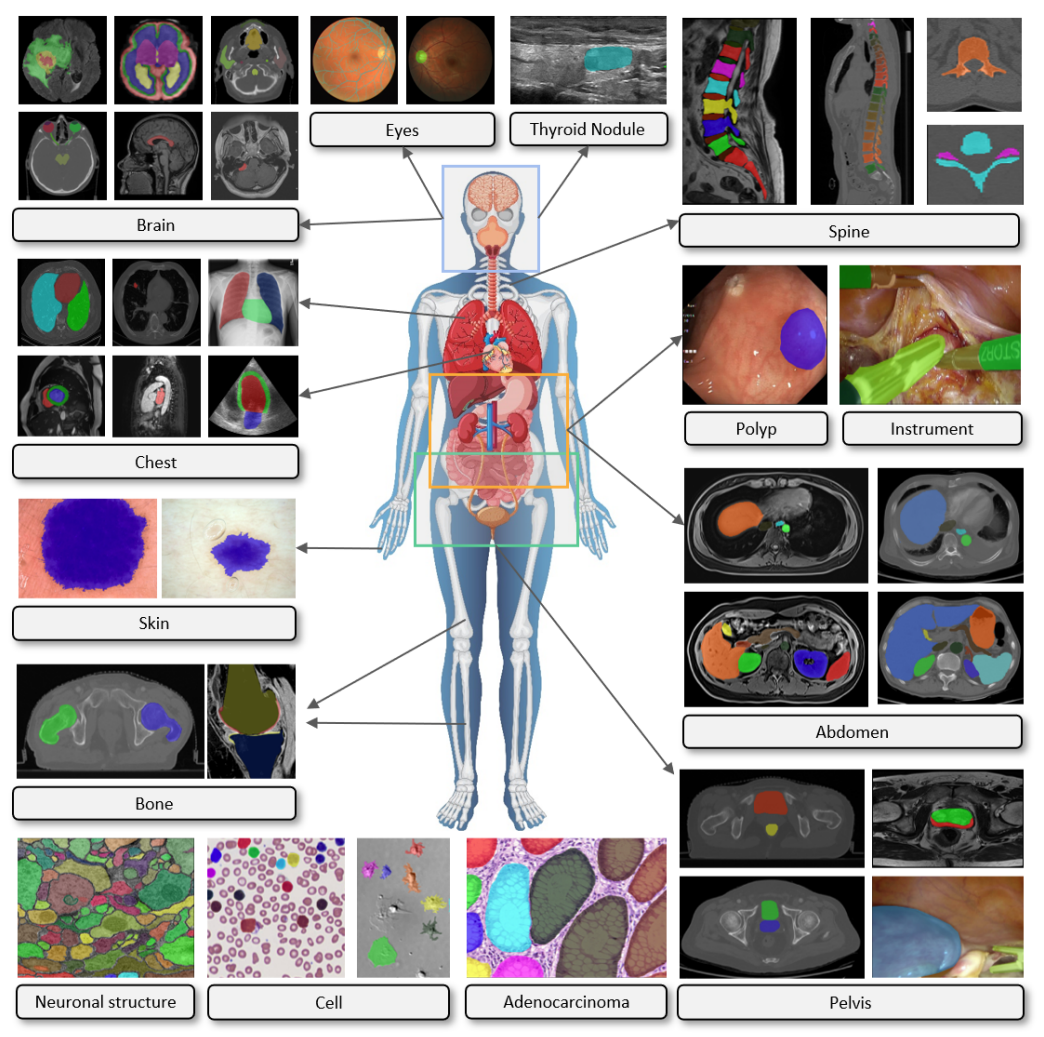
\includegraphics[width=\linewidth]{figures/fig4.png}
			\end{figure}
		\end{column}
		\begin{column}{0.5\linewidth}
			\begin{block}{疾病检测}
				AI可以辅助医生分析CT或X光图像, 帮助发现异常区域.
			\end{block}
			\begin{block}{疾病筛查}
				例如英国一些医院利用AI分析眼底图像, 帮助筛查糖尿病视网膜病变.
			\end{block}
			\begin{block}{病理分析}
				AI还可以帮助医生更快地分析显微镜下的组织切片, 提高效率.
			\end{block}
		\end{column}
	\end{columns}
\end{frame}

\begin{frame}
	\frametitle{智能交通系统}
	\begin{columns}
		\begin{column}{0.6\linewidth}
			\begin{figure}
				\centering
				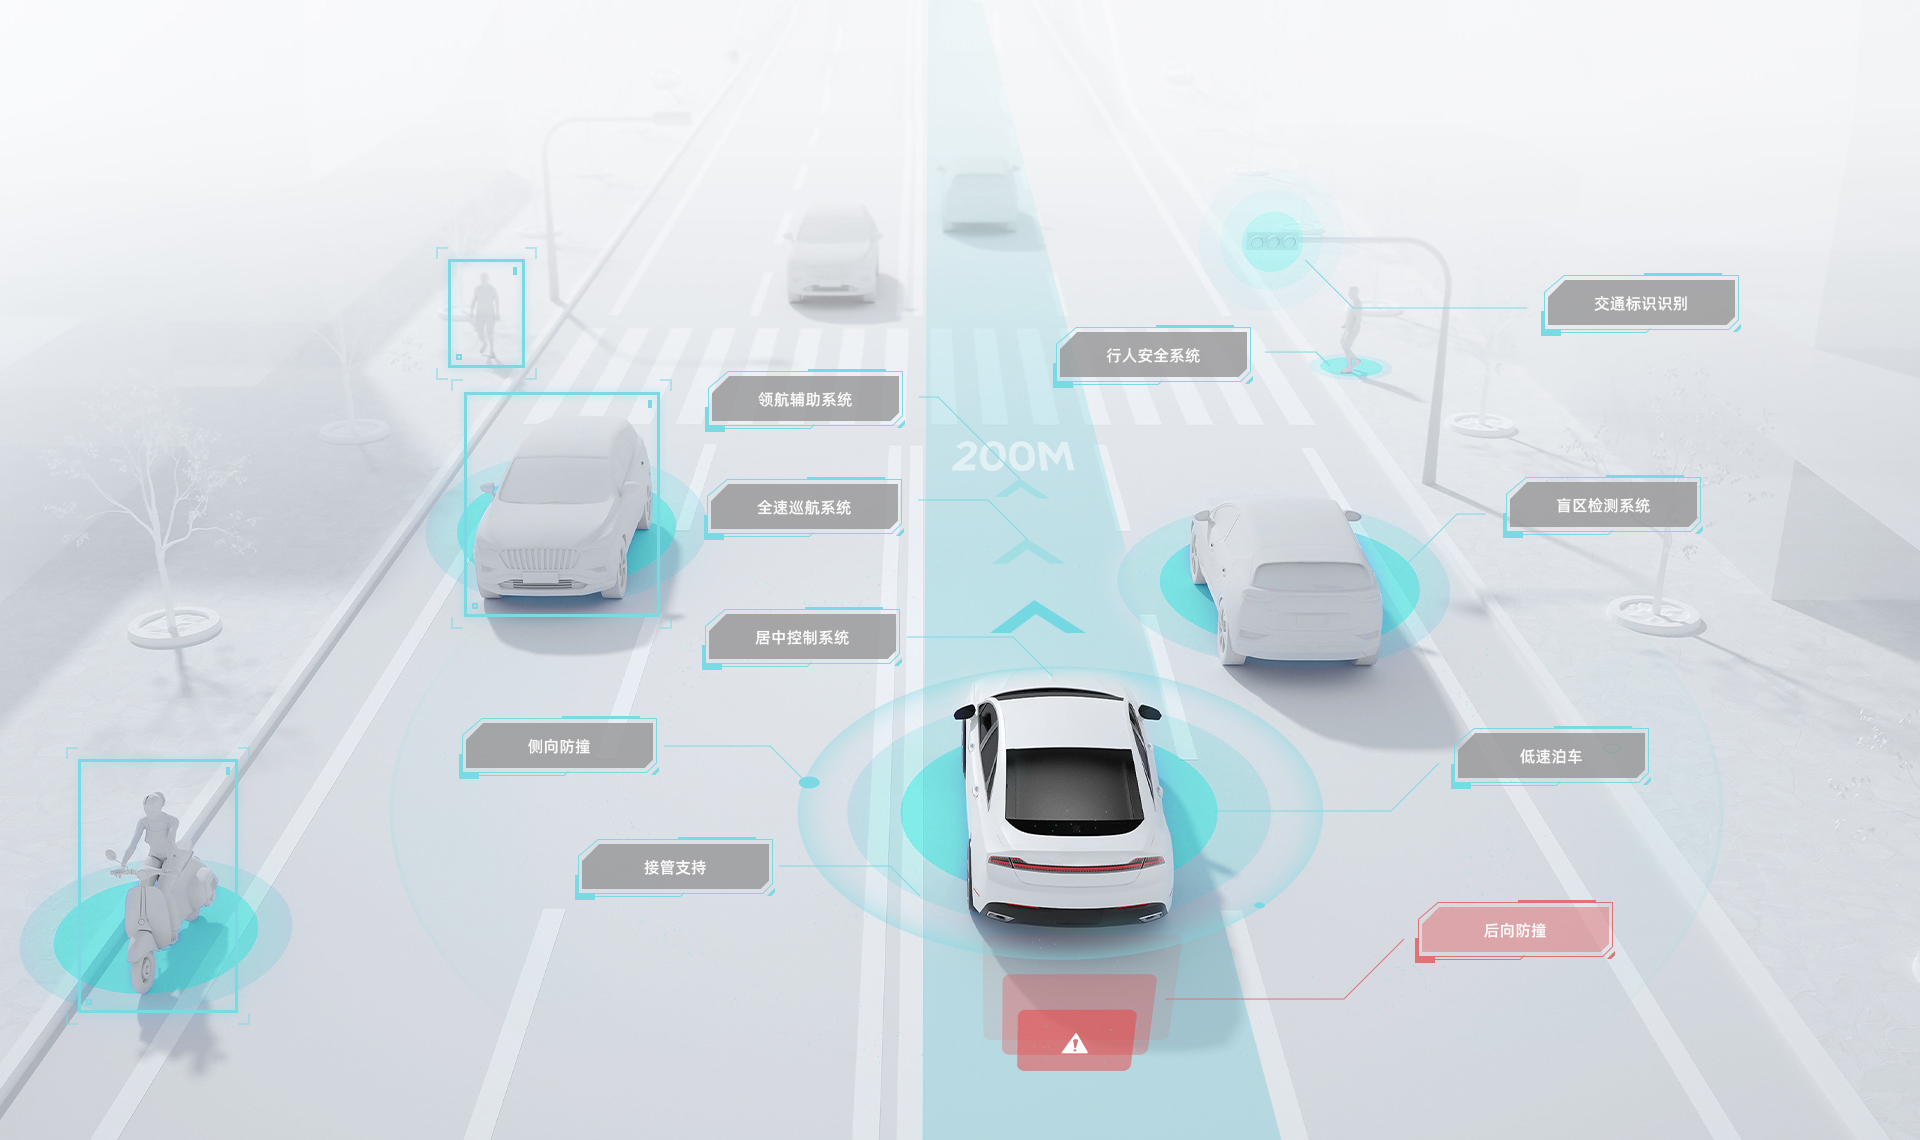
\includegraphics[width=\linewidth]{figures/fig5.png}
			\end{figure}
		\end{column}
		\begin{column}{0.4\linewidth}
			\begin{block}{车辆识别}
				通过摄像头识别车牌和车辆类型, 用于交通管理.
			\end{block}
			\begin{block}{自动驾驶}
				自动驾驶汽车需要通过图像识别技术理解道路环境, 例如识别车道线和行人.
			\end{block}
			\begin{block}{交通安全预警}
				系统可以检测行人或自行车, 从而帮助减少交通事故.
			\end{block}
		\end{column}
	\end{columns}
\end{frame}

\begin{frame}
	\frametitle{人脸识别}
	\begin{columns}
		\begin{column}{0.6\linewidth}
			\begin{figure}
				\centering
				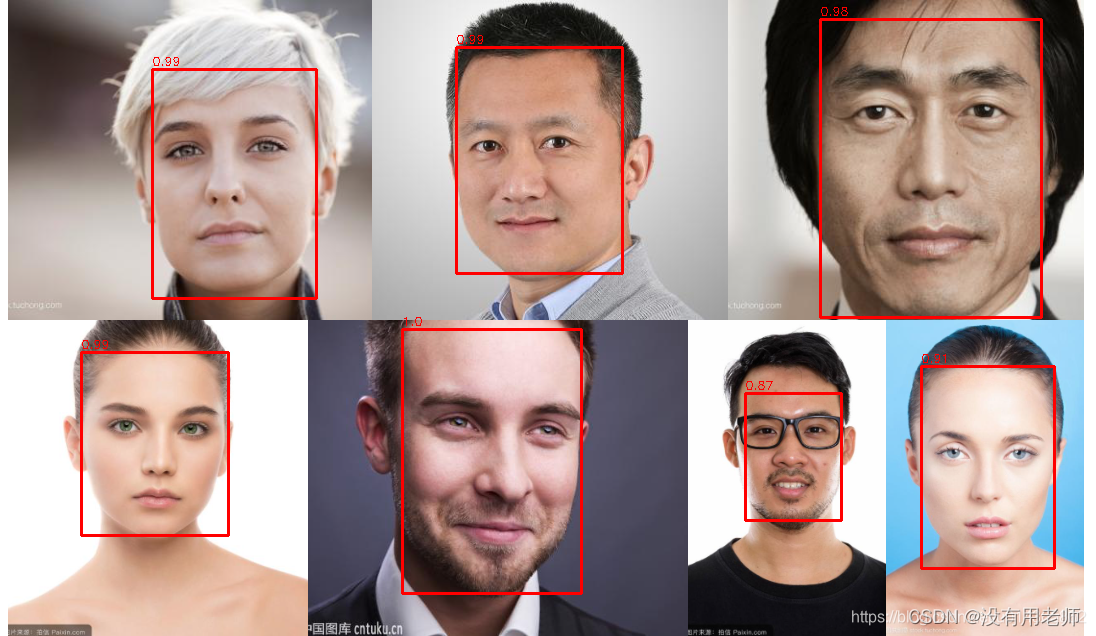
\includegraphics[width=\linewidth]{figures/fig6.png}
			\end{figure}
		\end{column}
		\begin{column}{0.4\linewidth}
			\begin{block}{身份验证}
				手机解锁, 门禁系统, 移动支付等场景广泛使用人脸识别完成身份认证, 例如Face ID.
			\end{block}
			\begin{block}{安防布控}
				在机场, 车站等公共场所识别重点人员, 协助警方快速定位目标.
			\end{block}
			\begin{block}{活体检测}
				通过分析眨眼, 头部转动等动作判断是否为真人, 防止照片或视频伪造攻击.
			\end{block}
		\end{column}
	\end{columns}
\end{frame}

\section[未来趋势]{AI图像识别的未来趋势}

\begin{frame}
	\frametitle{太空探索}

	\begin{figure}
		\centering
		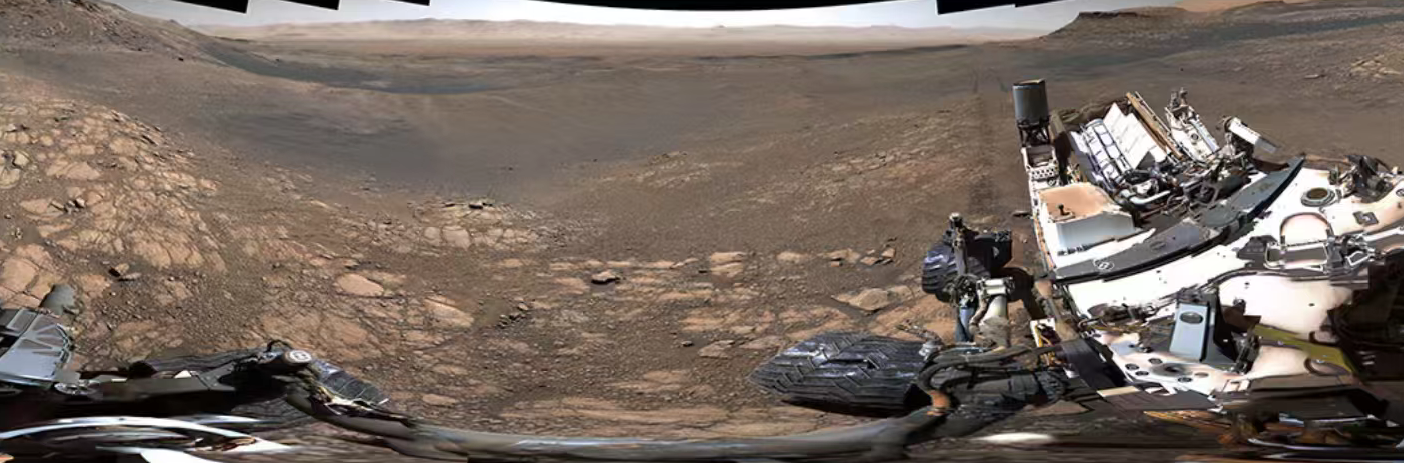
\includegraphics[width=0.7\linewidth]{figures/fig7.png}
	\end{figure}
	\begin{columns}[t]
		\begin{column}{0.3\linewidth}
			\begin{block}{自主导航}
				实时识别岩石, 沙丘, 陡坡等障碍,
				为火星车规划安全行驶路径.
			\end{block}
		\end{column}
		\begin{column}{0.3\linewidth}
			\begin{block}{科学目标识别}
				自动分类与标记具有特殊纹理或颜色的岩石,
				辅助科学家锁定高价值科学目标.
			\end{block}
		\end{column}
		\begin{column}{0.3\linewidth}
			\begin{block}{自我状态检测}
				视觉检测探测器本体 (如车轮, 机械臂) 的状态,
				实现自主健康监控.
			\end{block}
		\end{column}
	\end{columns}
\end{frame}

\begin{frame}
	\frametitle{文物保护}
	\begin{columns}
		\begin{column}{0.6\linewidth}
			\begin{figure}
				\centering
				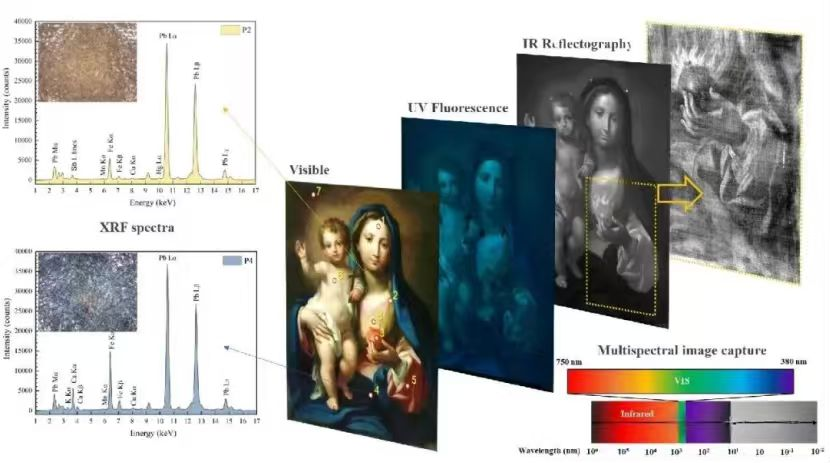
\includegraphics[width=\linewidth]{figures/fig8.jpg}
			\end{figure}
		\end{column}
		\begin{column}{0.4\linewidth}
			\begin{block}{多光谱成像分析}
				通过可见光, 紫外荧光, 红外反射等多光谱成像,
				结合X射线荧光光谱 (XRF) 分析,
				实现对画作颜料成分, 底层底稿及修复痕迹的无损检测.
			\end{block}
			\begin{block}{科学价值}
				识别颜料元素分布, 隐藏构图和画作状态,
				为文物真伪鉴定, 创作技法研究和修复保护提供科学依据,
				大幅提升艺术品分析的精度与效率.
			\end{block}
		\end{column}
	\end{columns}
\end{frame}

\begin{frame}
	\frametitle{动物监测}
	\begin{columns}[t]
		\begin{column}{0.5\linewidth}
			\begin{block}{陆地动物识别}
				在复杂背景中精准检测与分类羚羊, 狐狸, 牛等多类陆地动物,
				通过目标框与关键点标注实现物种识别,
				为野生动物监测提供高效手段.
				\begin{figure}
					\centering
					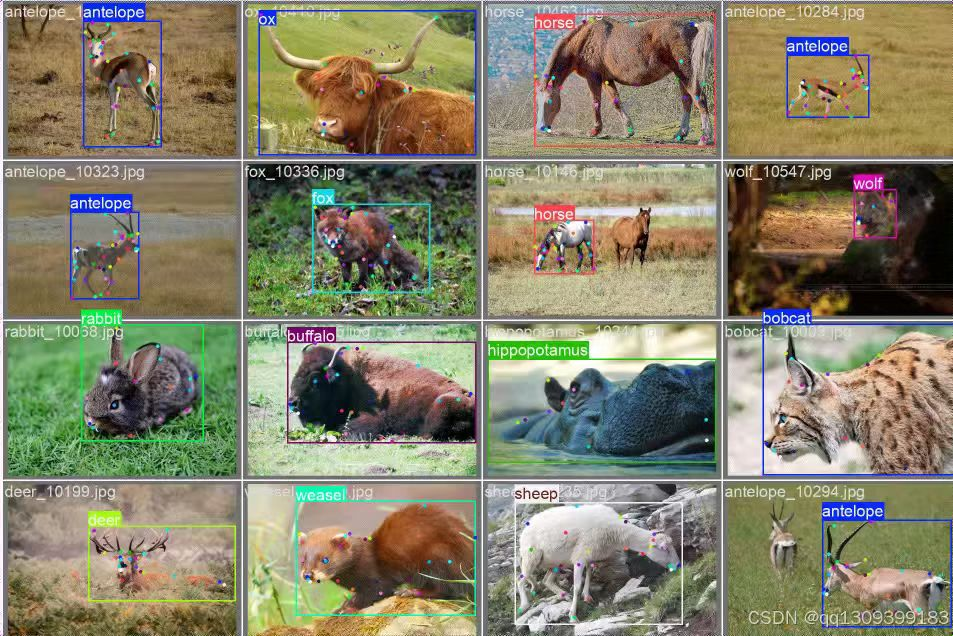
\includegraphics[width=0.7\linewidth]{figures/fig9.jpg}
				\end{figure}
			\end{block}
		\end{column}
		\begin{column}{0.5\linewidth}
			\begin{block}{水下生物识别}
				在复杂水下环境中检测鱼类, 珊瑚及潜水员,
				精准定位目标,
				为海洋生物调查与水下生态监测提供自动化技术支持.
				\begin{figure}
					\centering
					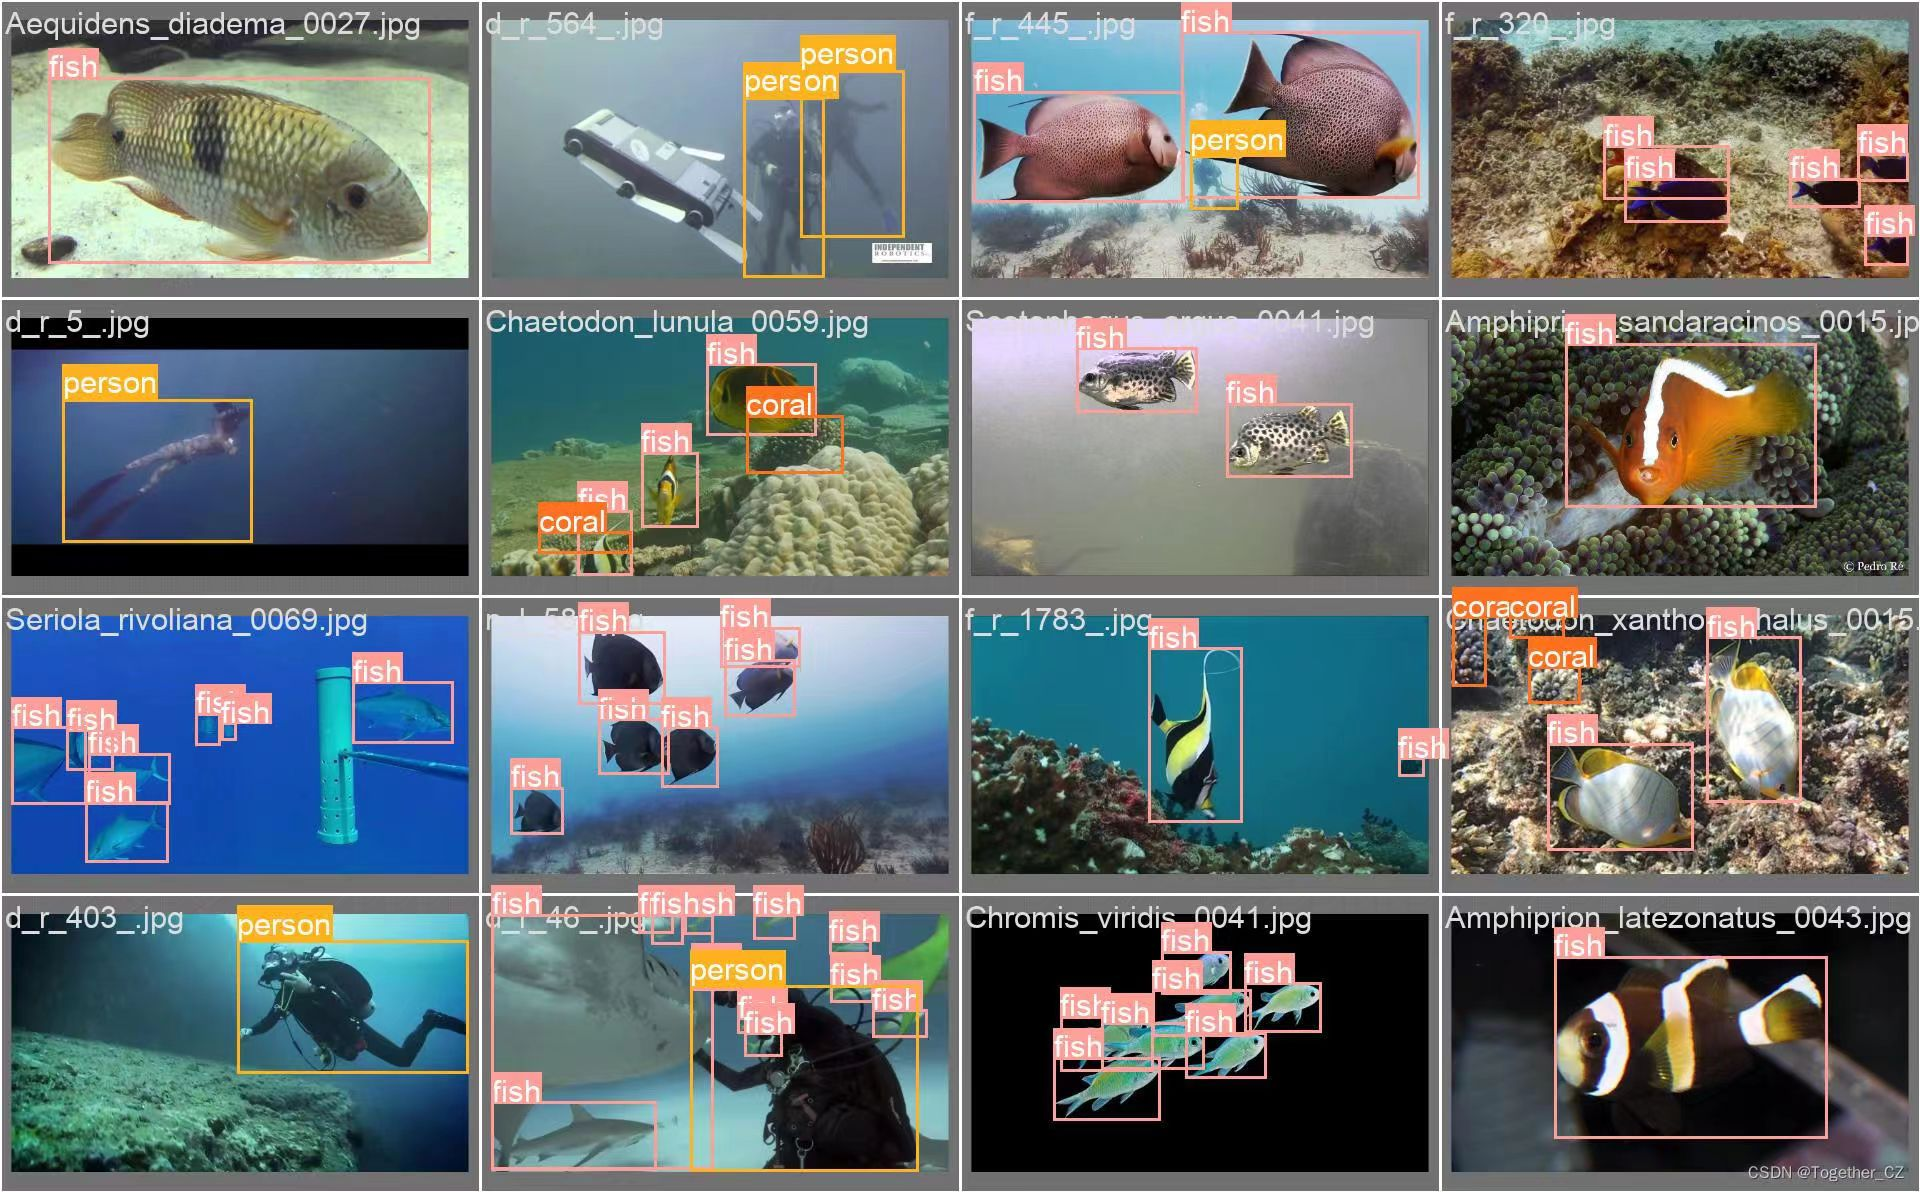
\includegraphics[width=0.7\linewidth]{figures/fig10.jpg}
				\end{figure}
			\end{block}
		\end{column}
	\end{columns}
\end{frame}

\section[社会安全]{AI图像识别的社会安全}

\begin{frame}
	\frametitle{身份伪装与欺诈}
	\begin{columns}
		\begin{column}{0.5\linewidth}
			\begin{figure}
				\centering
				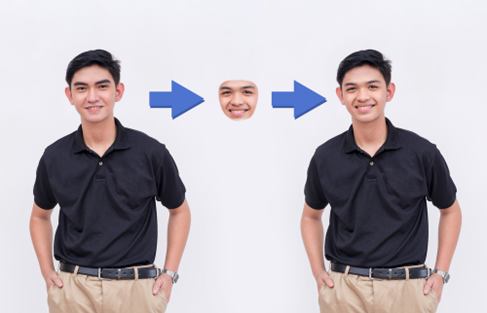
\includegraphics[width=\linewidth]{figures/fig11.png}
			\end{figure}
			深度伪造 (Deepfake) 技术让身份冒充的门槛大幅降低, 无需专业技能即可完成换脸与拟声, 成为实施新型欺诈的核心工具.
		\end{column}
		\begin{column}{0.5\linewidth}
			\begin{block}{金融诈骗}
				伪造企业高管视频下达转账指令, 或冒充亲友进行电信诈骗, 给企业和个人带来巨大的经济损失.
			\end{block}
			\begin{block}{名誉损害}
				恶意合成虚假不雅或不当言论视频, 这种数字栽赃能在短时间内摧毁个人声誉与品牌公信力.
			\end{block}
		\end{column}
	\end{columns}
\end{frame}

\begin{frame}
	\frametitle{大规模监控与隐私泄露}
	\begin{columns}
		\begin{column}{0.5\linewidth}
			\begin{figure}
				\centering
				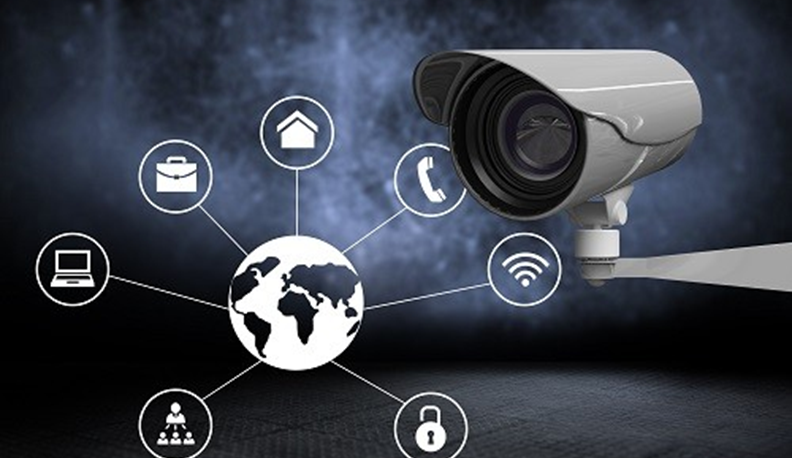
\includegraphics[width=\linewidth]{figures/fig12.png}
			\end{figure}
			无处不在的高清摄像头与 AI 识别算法相结合, 使对特定个体的大规模, 低成本, 实时追踪成为常态, 个人的不可见性在技术面前逐渐消失.
		\end{column}
		\begin{column}{0.5\linewidth}
			\begin{block}{隐私全面暴露}
				行踪, 行为乃至微表情被无孔不入地捕捉, 私人生活的透明度被无限放大.
			\end{block}
			\begin{block}{生物特征数据滥用}
				人脸, 虹膜等生物特征数据一旦泄露, 将直接关联个人身份, 这种不可逆的威胁对人身和财产安全影响深远.
			\end{block}
		\end{column}
	\end{columns}
\end{frame}

\begin{frame}
	\frametitle{公共安全与社会稳定威胁}
	\begin{columns}
		\begin{column}{0.5\linewidth}
			\begin{figure}
				\centering
				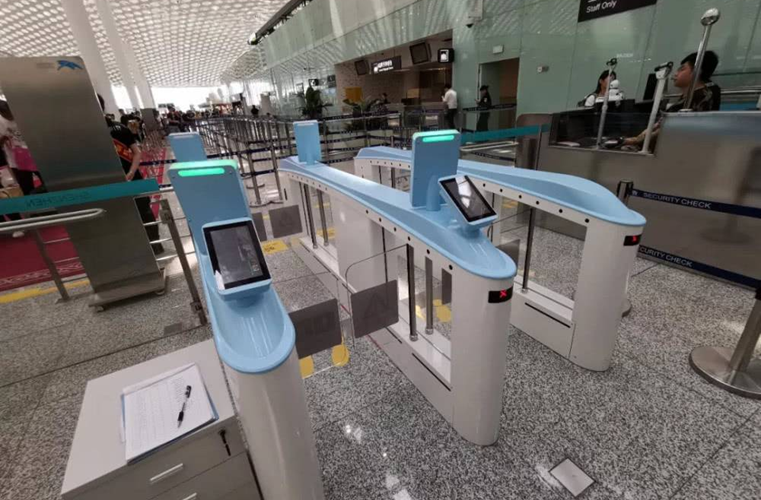
\includegraphics[width=\linewidth]{figures/fig13.png}
			\end{figure}
			当 AI 图像识别与生成技术被恶意滥用时, 不仅能规避常规安防检查, 更能通过制造虚假信息引发社会层面的连锁反应.
		\end{column}
		\begin{column}{0.5\linewidth}
			\begin{block}{躲避安防检查}
				利用 3D 面具或深度伪造复刻面部特征, 绕过机场, 车站等关键枢纽的人脸识别闸机.
			\end{block}
			\begin{block}{虚假信息煽动}
				生成高逼真度的虚假现场影像, 在公共网络空间快速传播, 极易激化群体对立情绪, 引发社会恐慌.
			\end{block}
		\end{column}
	\end{columns}
\end{frame}

\section{总结}

\begin{frame}
	\frametitle{总结}
	\begin{columns}[t]
		\begin{column}{0.3\linewidth}
			\begin{block}{技术核心}
				AI图像识别依靠深度神经网络, 通过层级特征学习和梯度下降算法, 从海量数据中自动提取从浅层到高层的视觉特征.
			\end{block}
		\end{column}
		\begin{column}{0.3\linewidth}
			\begin{block}{广泛应用}
				技术已在医疗影像诊断, 智能交通和人脸识别等领域取得了显著成果, 并加速向太空探索, 文物保护, 生态监测等前沿方向推进.
			\end{block}
		\end{column}
		\begin{column}{0.3\linewidth}
			\begin{block}{前景与挑战}
				市场高速增长, 技术创新活跃, 但同时也面临数据隐私, 算法偏见和对抗攻击等伦理与安全挑战.
			\end{block}
		\end{column}
	\end{columns}
\end{frame}

\section*{致谢}

\begin{frame}
	\frametitle{}
	\centering

	\Huge Thanks!
\end{frame}

\end{document}